% -*- coding: utf-8 -*-
%-------------------------designed by zcf--------------
\documentclass[UTF8,a4paper,10pt]{ctexart}
\usepackage[left=3.17cm, right=3.17cm, top=2.74cm, bottom=2.74cm]{geometry}
\usepackage{amsmath}
\usepackage{graphicx,subfig}
\usepackage{float}
\usepackage{cite}
\usepackage{caption}
\usepackage{enumerate}
\usepackage{booktabs} %表格
\usepackage{multirow}
\newcommand{\tabincell}[2]{\begin{tabular}{@{}#1@{}}#2\end{tabular}}  %表格强制换行
%-------------------------字体设置--------------
% \usepackage{times} 
\usepackage{ctex}
\setCJKmainfont[ItalicFont=Noto Sans CJK SC Bold, BoldFont=Noto Serif CJK SC Black]{Noto Serif CJK SC}


\newcommand{\yihao}{\fontsize{26pt}{36pt}\selectfont}           % 一号, 1.4 倍行距
\newcommand{\erhao}{\fontsize{22pt}{28pt}\selectfont}          % 二号, 1.25倍行距
\newcommand{\xiaoer}{\fontsize{18pt}{18pt}\selectfont}          % 小二, 单倍行距
\newcommand{\sanhao}{\fontsize{16pt}{24pt}\selectfont}  %三号字
\newcommand{\xiaosan}{\fontsize{15pt}{22pt}\selectfont}        % 小三, 1.5倍行距
\newcommand{\sihao}{\fontsize{14pt}{21pt}\selectfont}            % 四号, 1.5 倍行距
\newcommand{\banxiaosi}{\fontsize{13pt}{19.5pt}\selectfont}    % 半小四, 1.5倍行距
\newcommand{\xiaosi}{\fontsize{12pt}{18pt}\selectfont}            % 小四, 1.5倍行距
\newcommand{\dawuhao}{\fontsize{11pt}{11pt}\selectfont}       % 大五号, 单倍行距
\newcommand{\wuhao}{\fontsize{10.5pt}{15.75pt}\selectfont}    % 五号, 单倍行距
%-------------------------章节名----------------
\usepackage{ctexcap} 
\CTEXsetup[name={,、},number={ \chinese{section}}]{section}
\CTEXsetup[name={(,)},number={\chinese{subsection}}]{subsection}
\CTEXsetup[name={,.},number={\arabic{subsubsection}}]{subsubsection}
%-------------------------页眉页脚--------------
\usepackage{fancyhdr}
\pagestyle{fancy}
\lhead{\kaishu \leftmark}
% \chead{}
\rhead{\kaishu 计算机网络实验报告}
\lfoot{}
\cfoot{\thepage}
\rfoot{}
\renewcommand{\headrulewidth}{0.1pt}  
\renewcommand{\footrulewidth}{0pt}%去掉横线
\newcommand{\HRule}{\rule{\linewidth}{0.5mm}}%标题横线
\newcommand{\HRulegrossa}{\rule{\linewidth}{1.2mm}}
%-----------------------伪代码------------------
\usepackage{algorithm}  
\usepackage{algorithmicx}  
\usepackage{algpseudocode}  
\floatname{algorithm}{Algorithm}  
\renewcommand{\algorithmicrequire}{\textbf{Input:}}  
\renewcommand{\algorithmicensure}{\textbf{Output:}} 
\usepackage{lipsum}  
\makeatletter
\newenvironment{breakablealgorithm}
  {% \begin{breakablealgorithm}
  \begin{center}
     \refstepcounter{algorithm}% New algorithm
     \hrule height.8pt depth0pt \kern2pt% \@fs@pre for \@fs@ruled
     \renewcommand{\caption}[2][\relax]{% Make a new \caption
      {\raggedright\textbf{\ALG@name~\thealgorithm} ##2\par}%
      \ifx\relax##1\relax % #1 is \relax
         \addcontentsline{loa}{algorithm}{\protect\numberline{\thealgorithm}##2}%
      \else % #1 is not \relax
         \addcontentsline{loa}{algorithm}{\protect\numberline{\thealgorithm}##1}%
      \fi
      \kern2pt\hrule\kern2pt
     }
  }{% \end{breakablealgorithm}
     \kern2pt\hrule\relax% \@fs@post for \@fs@ruled
  \end{center}
  }
\makeatother
%------------------------代码-------------------
\usepackage{xcolor} 
\usepackage{listings} 
\usepackage{graphicx}
\lstset{ 
breaklines,%自动换行
basicstyle=\small,
escapeinside=``,
keywordstyle=\color{ blue!70} \bfseries,
commentstyle=\color{red!50!green!50!blue!50},% 
stringstyle=\ttfamily,% 
extendedchars=false,% 
linewidth=\textwidth,% 
numbers=left,% 
numberstyle=\tiny \color{blue!50},% 
frame=trbl% 
rulesepcolor= \color{ red!20!green!20!blue!20} 
}
%------------超链接----------
\usepackage[colorlinks,linkcolor=black,anchorcolor=blue]{hyperref}
%------------------------TODO-------------------
\usepackage{enumitem,amssymb}
\newlist{todolist}{itemize}{2}
\setlist[todolist]{label=$\square$}
% for check symbol 
\usepackage{pifont}
\newcommand{\cmark}{\ding{51}}%
\newcommand{\xmark}{\ding{55}}%
\newcommand{\done}{\rlap{$\square$}{\raisebox{2pt}{\large\hspace{1pt}\cmark}}\hspace{-2.5pt}}
\newcommand{\wontfix}{\rlap{$\square$}{\large\hspace{1pt}\xmark}}
%------------------------水印-------------------
\usepackage{tikz}
\usepackage{xcolor}
\usepackage{eso-pic}
\usepackage{verbatim}

\newcommand{\watermark}[3]{\AddToShipoutPictureBG{
\parbox[b][\paperheight]{\paperwidth}{
\vfill%
\centering%
\tikz[remember picture, overlay]%
  \node [rotate = #1, scale = #2] at (current page.center)%
    {\textcolor{gray!80!cyan!30!magenta!30}{#3}};
\vfill}}}
\lstset{
  basicstyle=\ttfamily\small, % 使用打字机字体并设置为小号
  numbers=left,
}
%———————————————————————————————————————————正文
%----------------------------------------------
\begin{document}
\begin{titlepage}
    \begin{center}
    
\includegraphics[width=0.8\textwidth]{NKU.png}\\[1cm]    
    \textsc{\Huge \kaishu{\textbf{南\ \ \ \ \ \ 开\ \ \ \ \ \ 大\ \ \ \ \ \ 学}} }\\[0.9cm]
    \textsc{\huge \kaishu{\textbf{网\ \ 络\ \ 空\ \ 间\ \ 安\ \ 全\ \ 学\ \ 院}}}\\[0.9cm]
    \textsc{\huge \kaishu{\textbf{计算机网络实验报告}}}\\[0.8cm]
    \HRule \\[0.9cm]
    { \LARGE \bfseries Lab2 网络抓包}\\[0.4cm]
    \HRule \\[2.0cm]
    \centering
    \textsc{\LARGE \kaishu{2113946\ \ \ 刘国民 }}\\[0.5cm]
    \textsc{\LARGE \kaishu{年级\ :\ 2021级}}\\[0.5cm]
    \textsc{\LARGE \kaishu{专业\ :\ 信息安全}}\\[0.5cm]
    \vfill
    {\Large \today}
    \end{center}
\end{titlepage}



\newpage
\tableofcontents
\setcounter{page}{1}

\vspace{1cm}

\section{实验介绍}
本次实验采用 XAMPP 软件来创建一个本地的 Web 服务器环境,XAMPP 是一个广泛使用的、免费且易于安装的 Apache 发行版。然后使用 HTML、CSS 和 JavaScript 编写了 Web 页面,该网页包含了简单的文本信息、图片、超链接和音频。最后再通过浏览器获取自己编写的 Web 页面,使用 Wireshark 捕获浏览器与 Web 服务器的交互过程,并对整个流程进行分析说明。\par





\vspace{1cm}
\section{实验原理}
首先我们对从输入网址按下回车到看到网页的过程做一个分析,经历的步骤如下:
\vspace{1cm}
\begin{enumerate}
\item  输入网址并回车\par
用户在浏览器的地址栏中输入网址并按下回车键,请求访问该URL
\item 域名解析(DNS查询)\par
首先,浏览器会检查自己的缓存中是否有该域名的 IP 地址记录。如果没有,它会请求操作系统检查其缓存。如果操作系统也没有这个记录,它会向配置的DNS服务器发起 DNS 查询。最后 DNS 服务器把该域名对应的 IP 地址返回给浏览器。本次实验中,因为是在同一主机上进行浏览器和服务器的通信,使用 localhost,属于进程间通信(IPC),故不需要使用DNS查询。
\item 建立 TCP 连接\par
三次握手:浏览器得到网站的IP地址后,会通过 TCP 协议向服务器发起连接,进行"三次握手"以建立 TCP 连接。
\item 浏览器发送HTTP请求\par
TCP 连接成功建立后,浏览器会构造一个 HTTP 的 GET 请求,请求输入网址 URL 所对应的内容。通过TCP连接,请求被发送到服务器。
\item 服务器处理请求\par
服务器接收到 HTTP 请求后,服务器端的 HTTP 服务(在本次实验中使用的 Apache)会处理这个请求。服务器可能会进行一系列的内部处理,如查询数据库、执行后端逻辑等,来生成 HTTP 响应。在本次实验中由于不涉及数据库的查询,请求的资源只是 HTML 文档,所以服务器不需要进行上述的内部处理。
\item 发送 HTTP 响应\par
服务器将响应数据封装成响应报文,通过TCP连接发送回浏览器。
\item 浏览器处理响应\par
浏览器对接收到的响应报文进行解析,把 HTML 代码转换为用户可以看到的格式化页面。而在 HTML 文件中可能会包含图片、音频、CSS 样式表、JavaScript 文件等外部资源,浏览器会根据 HTML 文件中的地址,继续发送请求来获取这些资源。
\item 渲染页面\par
最后浏览器会根据 HTML 和 CSS 定义渲染页面,并且最终在浏览器窗口中把页面显示给用户
\end{enumerate}

\vspace{1cm}
下面是本次实验涉及到的协议类型:

\subsection{HTTP协议}
HTTP(Hyper Text Transfer Protocol),全称超文本传输协议,是用于从万维网服务器传输超文本到本地浏览器的传送协议,属于一种应用层协议。HTTP为无状态协议,采用一发一收,一问一答的模式。下面是HTTP协议的传输模式:
\begin{figure}[H]
    \centering
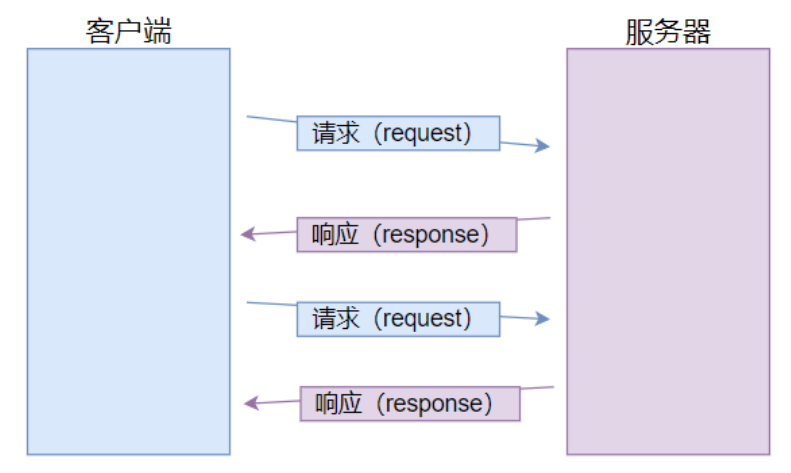
\includegraphics[width=0.4\textwidth]{img/HTTP协议模式.png}
    \caption{HTTP协议模式}
\end{figure}
HTTP协议有 HTTP1.0 、HTTP1.1 等不同版本。差异如下:
\begin{figure}[H]
    \centering
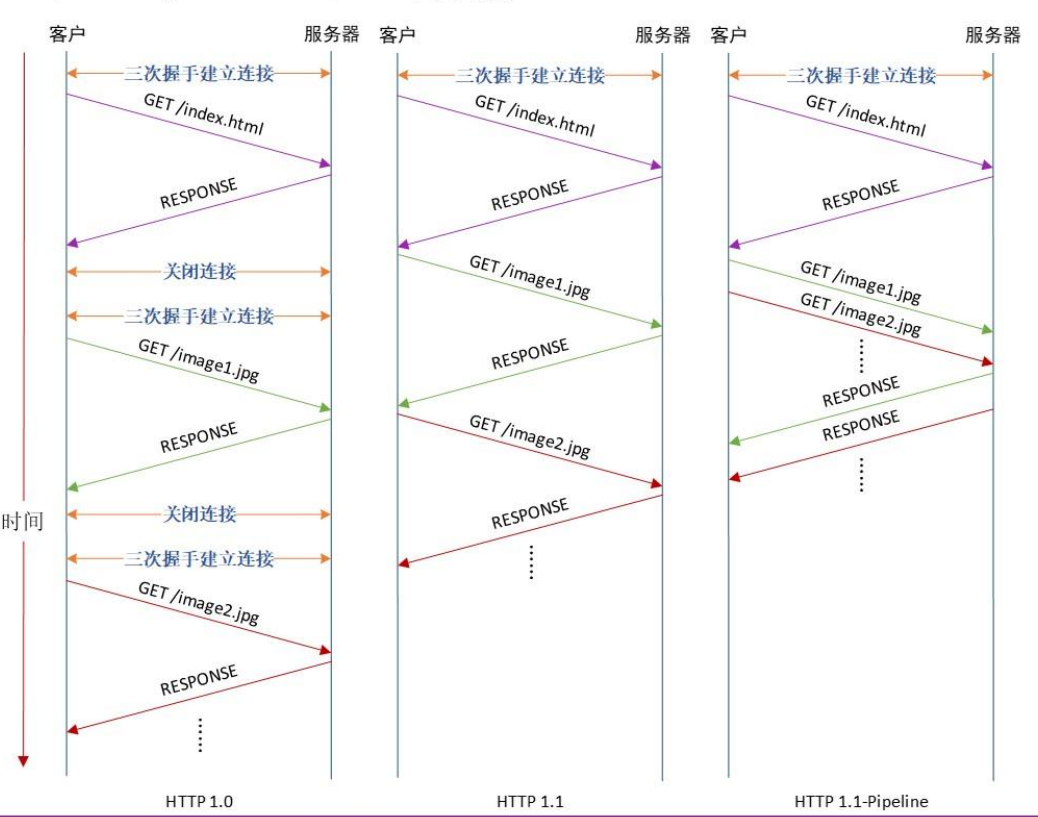
\includegraphics[width=0.4\textwidth]{img/HTTP比较.png}
    \caption{HTTP比较}
\end{figure}
从上图可以看到,在 HTTP1.0 中每一次客户端向服务端请求内容的时候,都需要重新建立 TCP 连接,而在 HTTP1.1 中,成功建立 TCP 连接后可以多次请求服务端资源,而流水线机制则可以在没有收到响应的时候继续请求资源。\par
\vspace{1cm}
HTTP 有请求和响应两种类型的报文格式,下面是请求报文的格式:
\begin{itemize}
\item 请求行:包含 HTTP 方法、请求的资源的 URL 以及 HTTP 版本。
\item 请求头:包含了关于请求的元数据,如客户端类型、接受的内容类型等,以键值对的方式显示。
\item 空行:请求头部和消息体之间必须有一个空行。
\item 消息体(可选):数据部分,通常在 POST 和 PUT 请求中用来发送表单数据或文件上传。 
\end{itemize}\par
\vspace{1cm}
下面是响应报文的格式:
\begin{itemize}
\item 响应行:包括 HTTP 版本、状态码和状态消息。
\item 响应头:包含有关服务器的信息以及进一步的请求说明。
\item 空行:头部和响应正文之间的一个空行。
\item 响应体:返回给客户端的实际数据。例如请求的 HTML 文档
\end{itemize}


\subsection{TCP协议}

TCP(Transmission Control Protocol) 是一种可靠的、面向连接的传输层通信协议,它确保在网络中的两个端点(通常是计算机)之间可靠地传输数据,是互联网协议套件的核心协议之一。其主要特点如下:
\begin{itemize}

\item 面向连接:在数据传输开始之前,TCP 需要源和目标之间建立连接,通过“三次握手”的过程完成的。

\item 可靠传输:TCP 通过序列号、确认响应和校验和等机制,确保数据正确无误地从源传送到目标。

\item 流量控制:TCP 使用窗口大小来控制发送方的数据传输速率,避免发送方过快地发送数据,导致接收方来不及处理。

\item 拥塞控制:TCP 还具有拥塞控制机制,如慢启动、拥塞避免、快速重传和快速恢复,以适应网络条件,避免网络拥塞。

\item 数据流:TCP 提供可靠字节流服务,无需关心数据报文的边界。

\item 全双工通信:TCP 允许双方在连接中同时发送和接收数据。

\item 多路复用:多个 TCP 连接可以同时在一个网络接口上运作,每个连接由一个唯一的源 IP/端口和目标 IP/端口对标识。

\end{itemize}





\subsubsection{TCP三次握手}
TCP 三次握手用于在两个网络设备之间建立一个可靠的连接。它涉及到序列号的同步和确认机制,确保双方都准备好进行数据传输。下面是三次握手的详细流程:
\begin{enumerate}

\item 第一次握手:SYN\par
握手开始时,客户端选择一个初始序列号(ISN: Initial Sequence Number)并向服务器发送一个 SYN (同步序列编号)标志设置为1的 TCP 段,表示客户端打算建立连接。这个 SYN 包中不包含应用层数据。

\item 第二次握手:SYN + ACK \par
服务器准备好接受客户端的连接后,会发送一个 SYN 标志和 ACK(确认)标志都设置为1的TCP段回客户端,该 TCP 段的确认号 ACK 被设置为客户端的 ISN 加1,表示服务器已经收到了客户端的SYN包,并且同意建立连接。同时,服务器也选择自己的一个 ISN,将 TCP 包发送给客户端。 

\item 第三次握手:ACK \par
客户端接收到服务器的 SYN+ACK 包后,知道服务器已经准备好进行通信。客户端确认服务器 TCP 段的序列号是自己的 ISN + 1 后,将 ACK 确认号设置为服务器的 ISN 加1,然后发送给服务端。服务器收到这个 ACK 包后,就知道双方的初始序列号都被成功确认。至此,三次握手成功完成。

\end{enumerate}
三次握手图示如下:
\begin{figure}[H]
    \centering
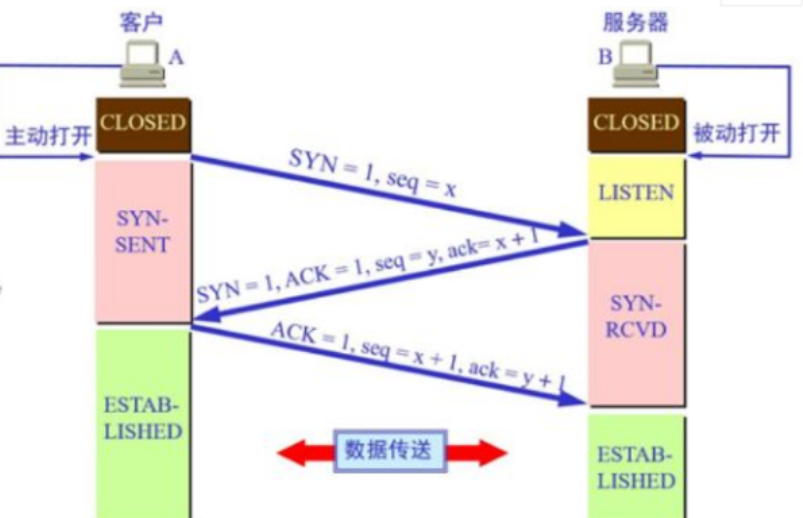
\includegraphics[width=0.4\textwidth]{img/三次握手图示.png}
    \caption{三次握手图示}
\end{figure}

完成这三次握手后,客户端与服务器之间建立了一个可靠的连接通道,可以开始进行数据传输。这个过程确保了双方都有能力发送和接收信息,并且同步了它们的序列号,这是TCP提供可靠传输服务的基础。

\subsubsection{TCP四次挥手}
TCP 使用"四次挥手"终止连接,这个过程需要四个步骤来确保双方都明确连接已经关闭。步骤如下:
\begin{enumerate}

\item 发起关闭\par
客户端决定关闭连接,发送一个 FIN 标志的报文给服务器。此时,客户端进入 FIN\_WAIT\_1 状态。FIN报文表示客户端已经没有数据发送了,但是还能接收数据。

\item 确认并等待关闭\par
服务器接收到 FIN 报文后,发送一个 ACK 报文作为响应,并进入 CLOSE\_WAIT 状态。此时,服务器仍然可以发送数据给客户端。客户端接收到 ACK 后,进入FIN\_WAIT\_2状态,等待服务器端的 FIN 报文。

\item 发起关闭\par
服务器如果还有未完成的任务,会继续处理。处理完毕后,服务器发送一个 FIN 报文给客户端,请求关闭连接,此时服务器进入 LAST\_ACK 状态。这个 FIN 报文表明服务器已经没有数据发送了,但是还能接收数据。
\item 最终确认\par
客户端接收到服务器的 FIN 报文后,进入 TIME\_WAIT状态,然后发送一个 ACK 给服务器,确认收到服务器端的 FIN 报文。服务器接收到这个 ACK 后,就关闭连接,进入 CLOSED 状态。
客户端会等待一段时间(称为2MSL,Maximum Segment Lifetime)以确保服务器接收到确认报文,然后关闭连接,进入  CLOSED 状态。
\end{enumerate}
四次挥手中的"挥手"指的是发送FIN和ACK报文的动作。整个过程确保了双方都能够清楚地知道通信被终止。图示如下:
\begin{figure}[H]
    \centering
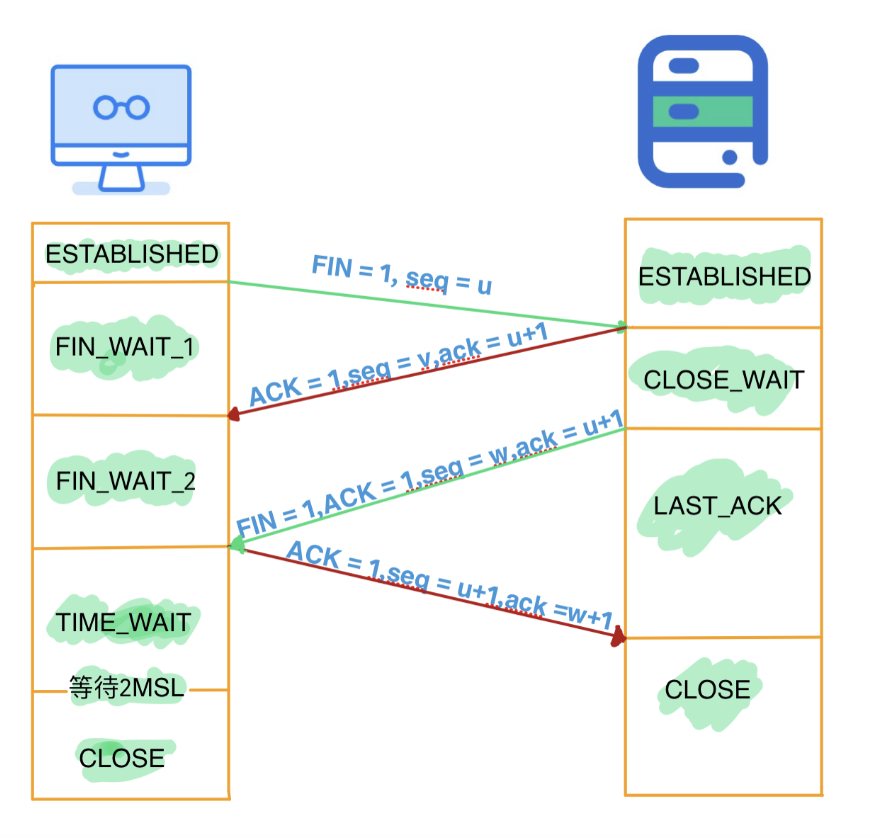
\includegraphics[width=0.4\textwidth]{img/四次挥手图示.png}
    \caption{四次挥手图示}
\end{figure}


\vspace{1cm}

\section{实验代码}

本次实验用 HTML、CSS 和 JavaScript 编写前端的网页代码。

\subsection{HTML文档}
源代码如下:
\begin{lstlisting}[frame=trbl,language={HTML}]
<!-- this is comment -->
<!DOCTYPE html>
<html lang="zh-CN">
    <head>
        <meta charset="UTF-8">
        <title>my website </title>
        <link rel="stylesheet" href="mywebsite.css">
        <link rel="icon" href="favicon.ico" type="image/x-icon">
        <link rel="stylesheet" href="https://fonts.googleapis.com/css?family=Sofia">
    </head>
    <body id="background">
        <div class="welcome">
            Welcome to my website!
            <img src="/img/mylogo.png" alt="Mylogo" width="100" style="margin-left: 80px;" >
        </div>
        <br/>
        <div class="intro">
            <div class="label">
                <button id="butt1">
                    姓名
                </button>
                <br/>
                <button id="butt2">
                    专业
                </button>
                <br/>
                <button id="butt3">
                    学号
                </button>
            </div>
            <div class="content">
                <p id="text1">刘国民</p>
                <p id="text2">信息安全</p>
                <p id="text3">2113946</p>
            </div>
            <div id="buttom">
                <a href="https://github.com/NKU-liu1114" target="_blank">github账号个人主页</a>
                <audio controls>
                    <source src="intro.mp3" type="audio/mpeg">
                    浏览器不支持 audio 元素。
                  </audio>
            </div>     
        </div>
        <script src="mywebsite.js"></script>
    </body>
</html>
\end{lstlisting}\par

\subsubsection{head部分}

在 head 部分声明了采用 UTF-8 编码方式,并列出了需要的其他外部资源,包括:
\begin{itemize}
\item 同一路径下的 CSS 样式表
\item 同一路径下的 icon 图标
\item 引用字体族的 URL
\end{itemize}


\subsubsection{body部分}
\noindent 总体的网页布局如下:\par
\vspace{ 0.3cm}
用一个背景图片覆盖整个网页。网页上方显示 "Welcome to my website!" 的提示语,右边显示LOGO图片。提示语下方用一个边框来包裹信息。边框左边是“姓名”、“专业”、“学号”三个按钮,点击后会在边框中部显示对应的信息。边框底部是 github 账号链接和个人介绍的音频。 \par
根据以上布局思路,选择用 <div> 容器来包裹相应内容,同时可以得到元素和标签之间的嵌套关系。
\begin{itemize}
\item 首先用 div 容器包裹欢迎语 "Welcome to my website!" ,并利用 <img> 标签插入了一个 LOGO。
\item 用 div 容器制作一个只有背景色的圆角边框,之后的元素都放在该容器中
\item 用 div 容器占据边框的左上部分,并在容器中插入三个 button ,用于配合 JavaScript 实现点击显示的功能。
\item 用 div 容器占据边框的右上部分,用于包裹点击显示后出现的文本信息。
\item 用 div 容器占据边框的底部,在 div 中放入超链接和音频。
\end{itemize}



\subsection{CSS样式表}
CSS 样式表如下:
\begin{lstlisting}[frame=trbl]
#background{
    background-image: url("img/mybackground.png");
    background-repeat: no-repeat;
    background-size: cover;
}
.welcome{
    font-family: "Sofia";
    font-size:60px;
    text-align:center;
    margin-top: 50px;
    margin-left: 200px;
    color:rgb(38, 147, 242);
}
.intro{
    background-color: rgb(133, 238, 152);
    opacity:0.5;
    height:500px;
    width:620px;
    margin-left: 430px; 
    border-radius: 8px;
    margin-top: 4px; 
    color:rgb(18, 127, 237);
}
.label{
    float:left;
    height:400px;
    width:200px;
}
#butt1{
    border-radius: 8px;
    font-family:"KaiTi";
    color:black;
    margin-top: 80px;
    margin-left:50px;
    transform: rotate(-20deg);
    font-size: 30px;

}
#butt2{
    border-radius: 8px;
    font-family:"KaiTi";
    color:black;
    margin-top: 80px;
    margin-left:50px;
    transform: rotate(-20deg);
    font-size: 30px;

}
#butt3{
    border-radius: 8px;
    font-family:"KaiTi";
    color:black;
    margin-top: 80px;
    margin-left:50px;
    transform: rotate(-20deg);
    font-size: 30px;

}
.content{
    width:380px;
    height: 360px;
    margin-left:200px;
    float:center;
    padding:30px;
}
#text1{
    visibility:hidden;
    color:black;
    font-size: 30px;
    font-family:"KaiTi";
    margin-top: 40px;
    font-weight: bold;
}
#text2{
    visibility:hidden;
    color:black;
    font-size: 30px;
    font-family:"KaiTi";
    margin-top: 90px;
    font-weight: bold;
}
#text3{
    visibility:hidden;
    color:black;
    font-size: 30px;
    font-family:"KaiTi";
    margin-top: 90px;
    font-weight: bold;
}
#buttom{
    font-family: "KaiTi";
    color:black;
    text-align: center;
    font-size: 20px;
    width:620px;
    height:80px;
}
\end{lstlisting}\par
根据网页设计的预期效果,对不同的 id 和 class 选择器配置相应的属性和值,其中的 id 和 class 与 HTML 中的相匹配。浏览器根据 CSS 文件来渲染页面,最后呈现在屏幕上。下面列出部分属性的含义:
\begin{itemize}
\item  margin-top:设置一个元素的上外边界
\item  font-family:指定文本的字体系列
\item  font-size:设置文本的字体大小
\item  width:指定元素内容区域的宽度
\item  border-radius:为元素创建圆角边框
\item  opacity:设置元素的不透明度
\item  ……
\end{itemize}
\subsection{Javascript脚本}
Javascript脚本如下:
\begin{lstlisting}[frame=trbl]
// 获取按钮和文本元素
var button1 = document.getElementById("butt1");
var button2 = document.getElementById("butt2");
var button3 = document.getElementById("butt3");
var text1 = document.getElementById("text1");
var text2 = document.getElementById("text2");
var text3 = document.getElementById("text3");
// 事件响应函数
function showMessage(text){
    // 显示文本元素
    if( text.style.visibility=="hidden"){
        text.style.visibility = "visible";
    }
    else{
        text.style.visibility = "hidden";
    }
}

// 为按钮添加点击事件监听器
button1.addEventListener("click", function() {
    showMessage(text1);
});
button2.addEventListener("click", function() {
    showMessage(text2);
});
button3.addEventListener("click", function() {
    showMessage(text3);
});
\end{lstlisting}
Javascript 用于增强网页的交互性。在本次实验中,当点击“姓名”、“学号”和“专业”的时候,才会显示相应的信息。所以我采用 Javascript 来实现。实现的原理是:为 "click" 这一动作绑定响应函数,再为每个按钮添加监听器。如果监听到这一动作,就进行相应函数的操作。\par
具体实现上,首先通过 getElementById() 函数来声明变量,之后声明响应函数,如果内容之前是被隐藏的,则更改它的属性为可见的;如果内容之前是被隐藏的,则更改它的属性为隐藏。然后再为三个按钮添加监听器即可。

\section{实验流程}
首先打开浏览器,打开 XAMPP,启动 Apache。
\begin{figure}[H]
    \centering
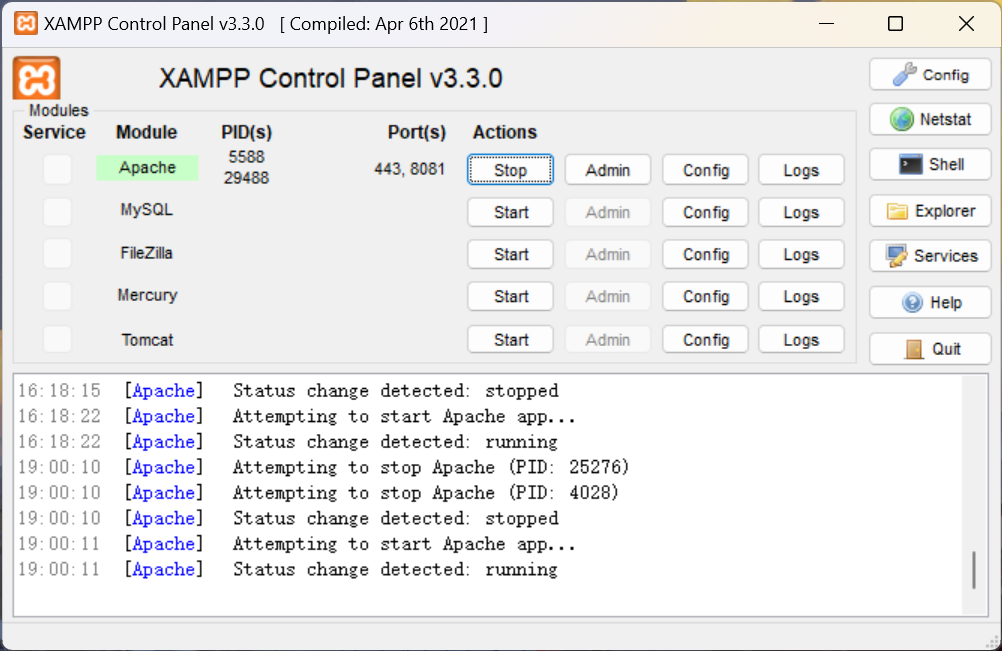
\includegraphics[width=0.6\textwidth]{img/Xampp启动.png}
    \caption{Xampp启动}
\end{figure}
从上图可以看到,端口号为8081,所以服务器的主机地址为:$localhost:8081$。之后打开 WireShark ,点击 Adapter for loopback traffic capture,用于捕获本地主机之间的网络通信。同时设置过滤:$tcp.port==8081$,准备抓包。
\begin{figure}[H]
    \centering
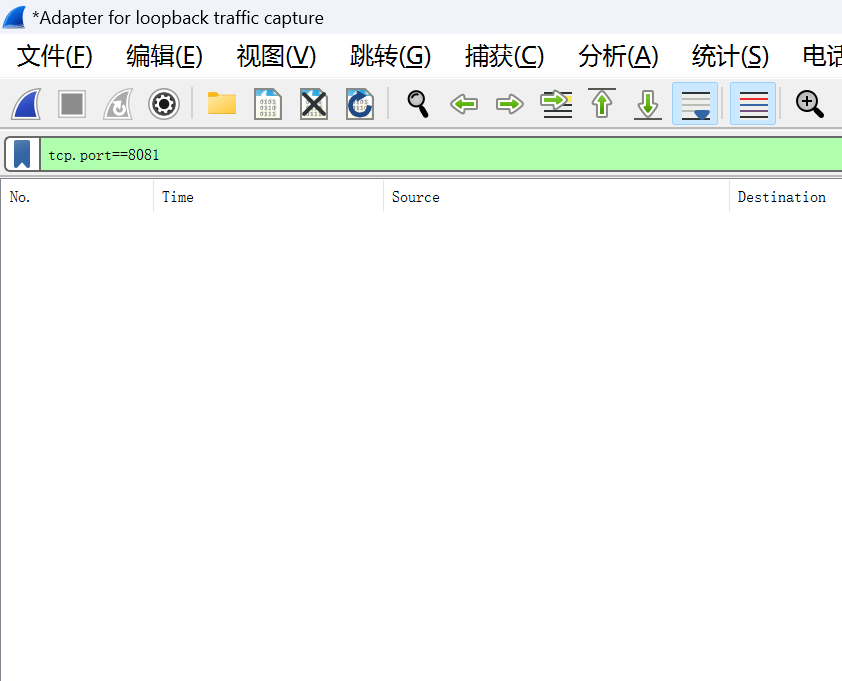
\includegraphics[width=0.6\textwidth]{img/WireShark初始化.png}
    \caption{WireShark初始化}
\end{figure}
设置成功后,点击开始,由于 XAMPP 软件的默认服务器资源在 htdocs 目录下,实验的代码、图片和音频放在 /htdocs/src 目录中,代开浏览器,输入 url: http://localhost:8081/src/mywebsite.html
\begin{figure}[H]
    \centering
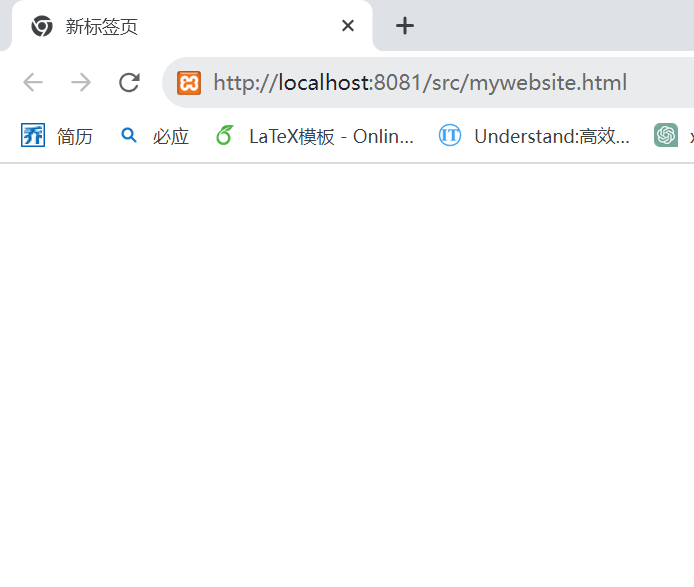
\includegraphics[width=0.4\textwidth]{img/URL.png}
    \caption{URL}
\end{figure}
之后按下 Enter 键,浏览器成功请求到服务端的资源,把 HTML 文档解释、渲染后显示在网页中,页面效果符合预期。
\begin{figure}[H]
    \centering
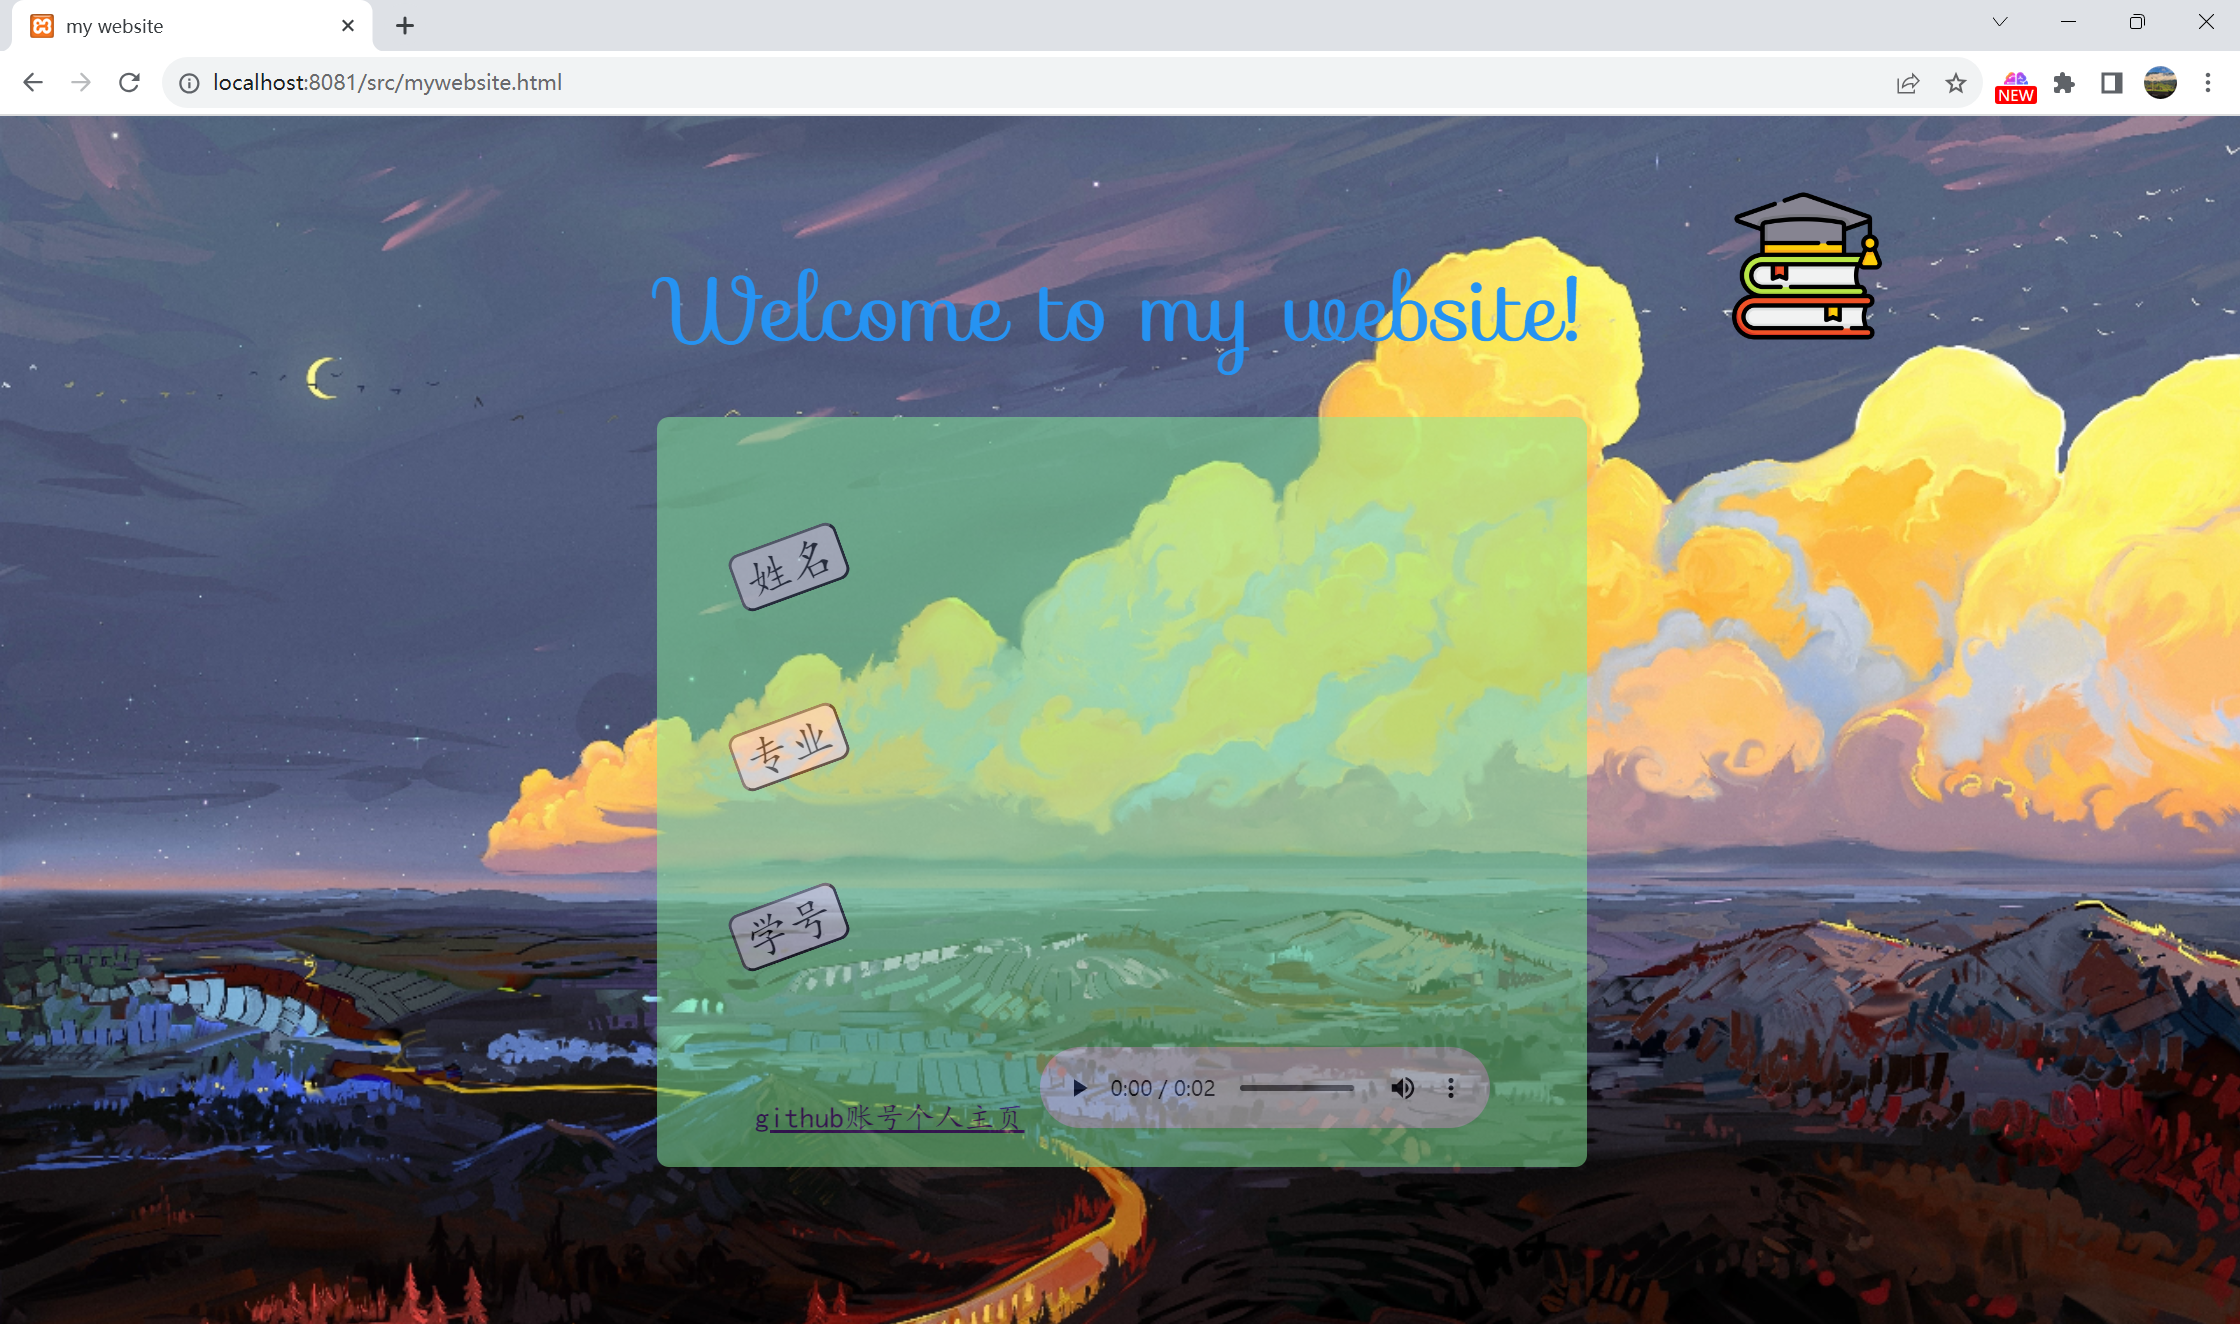
\includegraphics[width=0.8\textwidth]{img/网页界面.png}
    \caption{网页界面}
\end{figure}

我们点击三个按钮,可以看到成功显示相应的信息。其他的图片和音频信息也符合实验预期,说明浏览器成功拿到了需要的服务端资源。
\begin{figure}[H]
    \centering
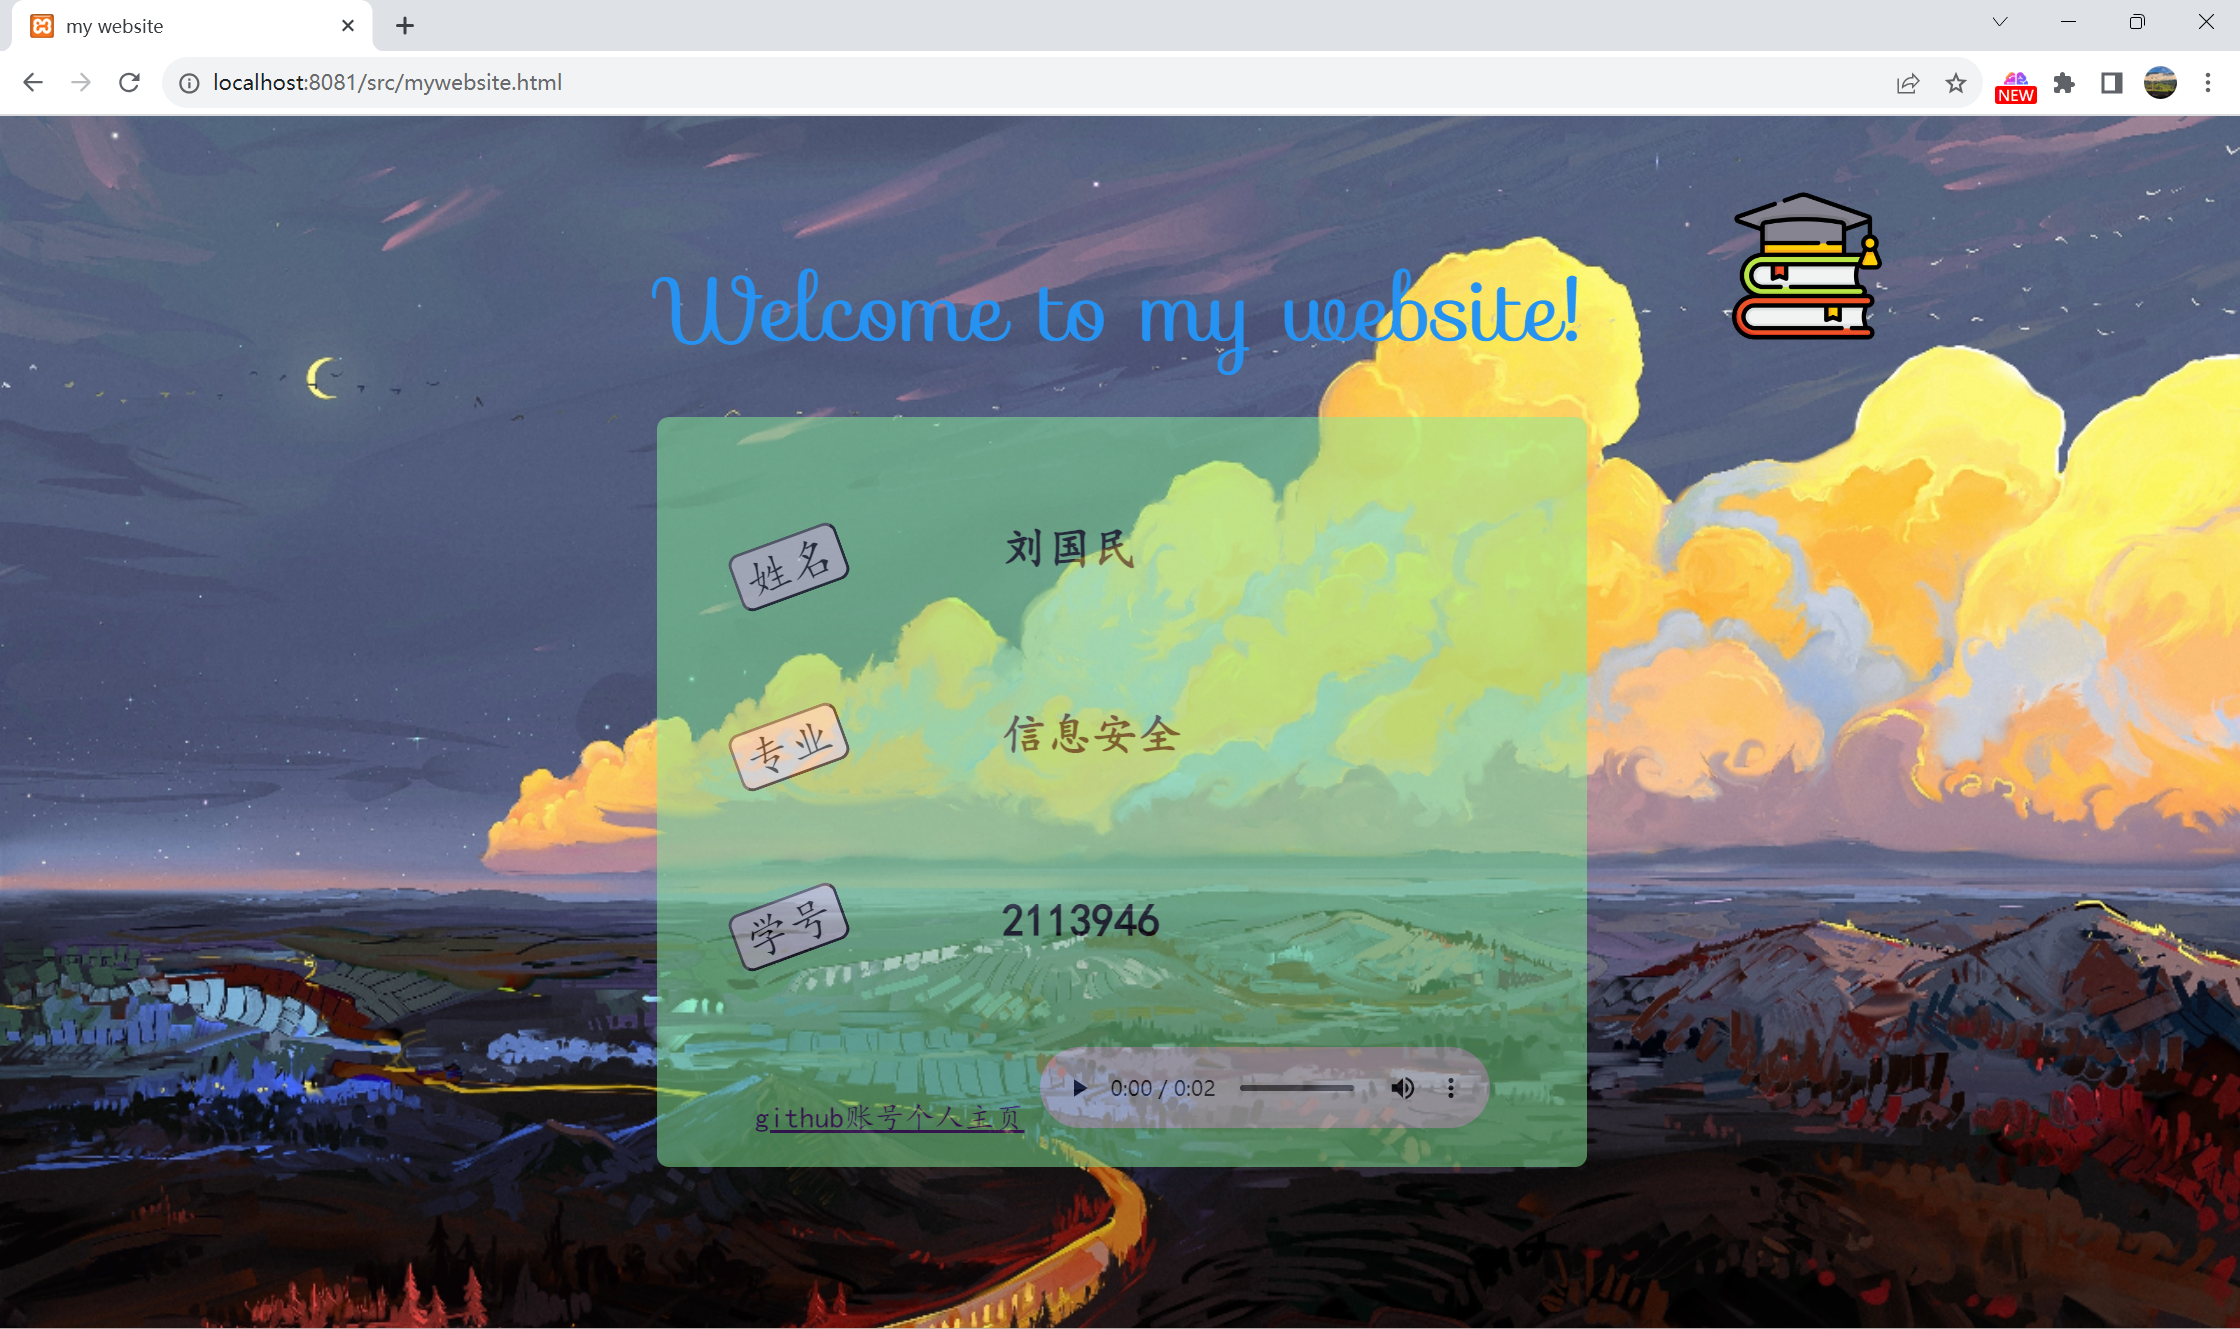
\includegraphics[width=0.8\textwidth]{img/显示信息.png}
    \caption{显示信息}
\end{figure}
至此,网页的分析完毕。下面对WireShark捕获到的数据包进行分析。可以看到如下界面:
\begin{figure}[H]
    \centering
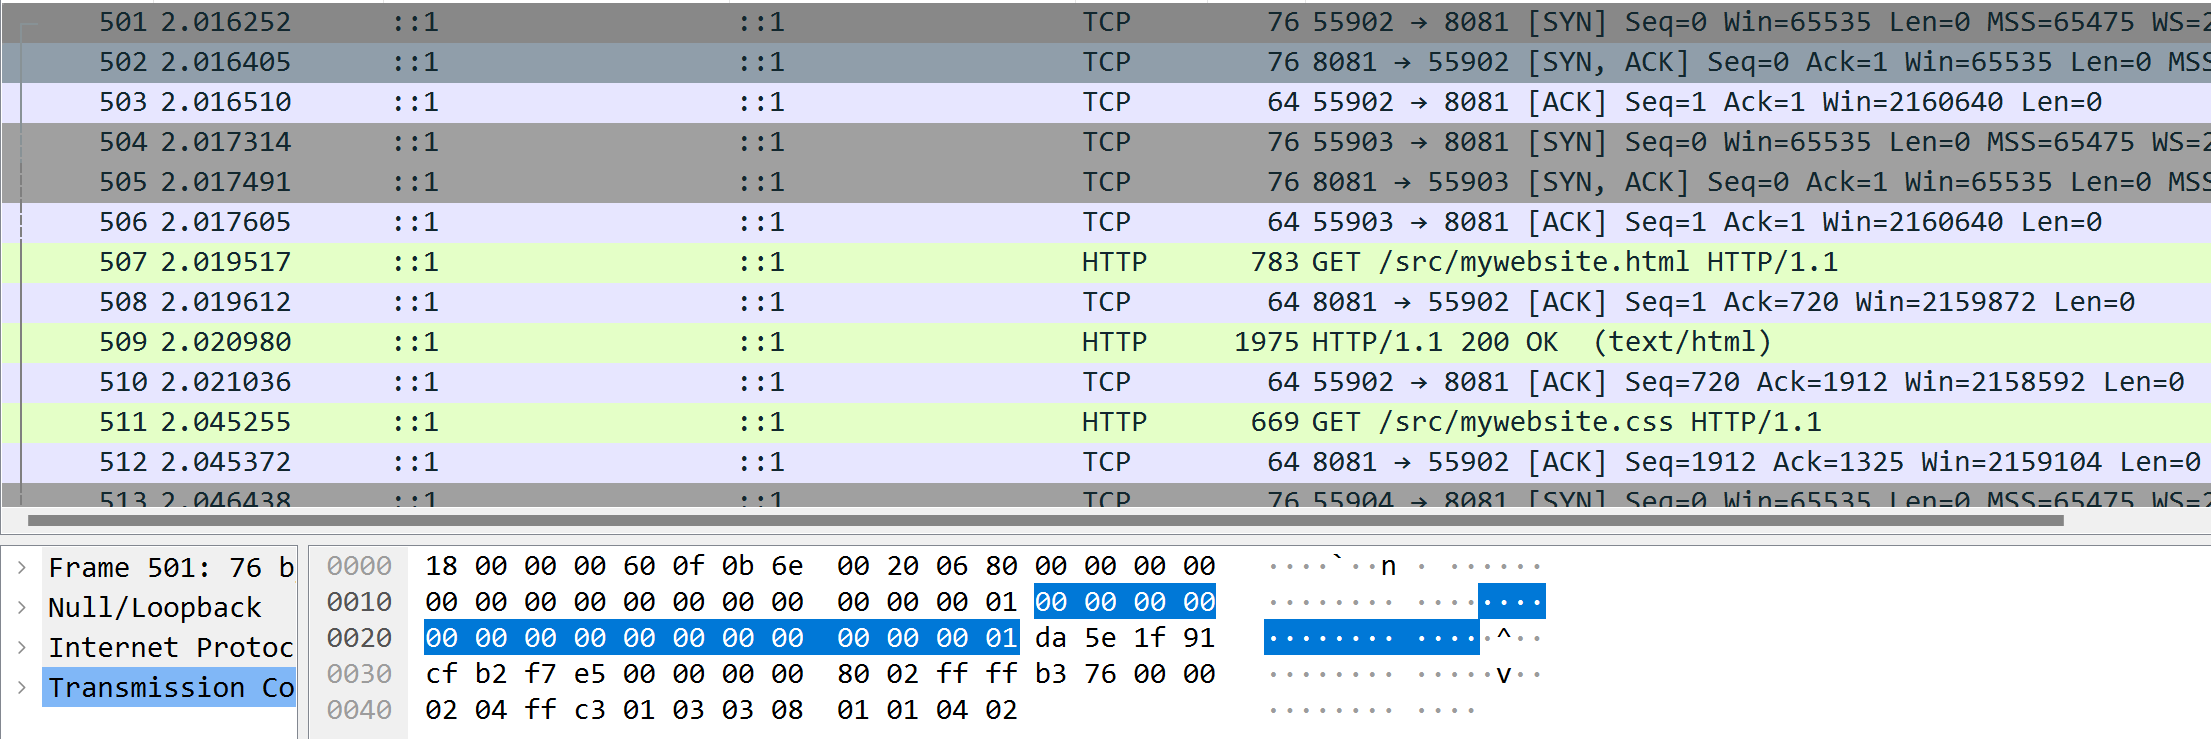
\includegraphics[width=1.0\textwidth]{img/三次握手.png}
    \caption{建立连接}
\end{figure}
首先可以看到 TCP 的三次握手。在这里我们发现浏览占用了两个端口,并分别建立 TCP 连接,这是因为浏览器为了加快资源的下载速度,同时占用了多个端口建立连接,下载所需资源。我们以其中一个端口(55902)为例来分析TCP 的三次握手。如上图所示,该端口首先向服务器端口8081发送一个 [SYN] 报文,请求建立连接。可以看到,这里的 Seq=0 ;服务器收到该报文返回一个 [SYN,ACK] 的报文,ACK 号为 1,表示收到了建立请求的报文,并设置自己的 Seq=0;最后客户端发给服务端一个 [ACK] 报文,表示收到该消息,此时 ACK=Seq=1 ,符合实验原理中叙述的过程,建立连接成功。\par
建立连接后,浏览器的占用的端口向服务端请求HTML资源,我们双击查看具体信息:
\begin{figure}[H]
    \centering
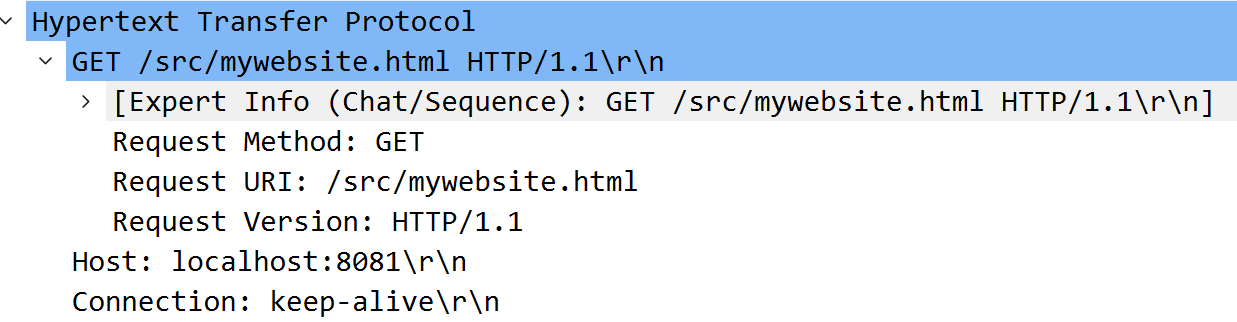
\includegraphics[width=0.6\textwidth]{img/HTTP请求.png}
    \caption{HTTP请求}
\end{figure}
从上图中可以看到,客户端发送的是 GET 请求,请求的是/src/mywebsite.html 资源,采用的是 HTTP 1.1 的协议类型,后续可以看到,该端口成功建立 TCP 连接后,再次请求资源的时候没有又一次进行三次握手的过程。客户端发送请求后,服务端发回了一个 ACK 的报文,表示已经收到该请求。双击打开服务端返回的响应报文,响应头和响应体符合响应报文的格式,返回的状态为200,代表成功拿到请求的资源,被请求的对象放在了响应体中。这里我们关注响应体的内容,即 原始的HTML 文档
\begin{figure}[H]
    \centering
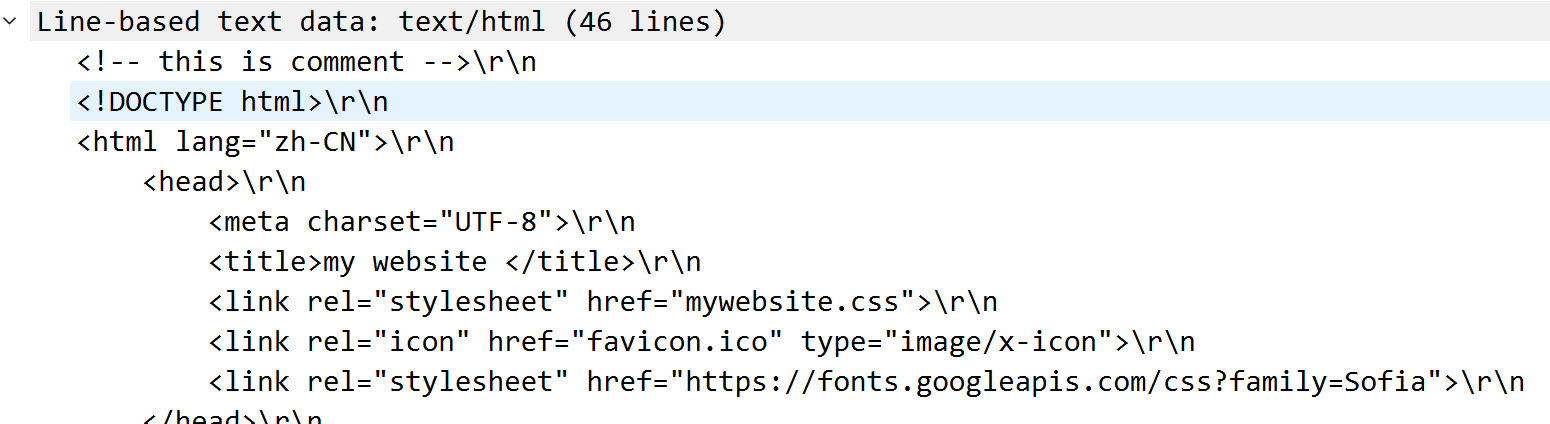
\includegraphics[width=0.6\textwidth]{img/HTTP响应体.png}
    \caption{HTTP响应体}
\end{figure}
在这里我注意到一个细节,HTML文档中注释等内容也被一并传回给了客户端,所以可以看到,对代码的预处理是在浏览器进行的。同时,在这里由于 HTML 文档中包含 图片、音频 和 CSS/Javascript 等代码文件,所以后续还需要继续发送请求拿到这些资源。
\begin{figure}[H]
    \centering
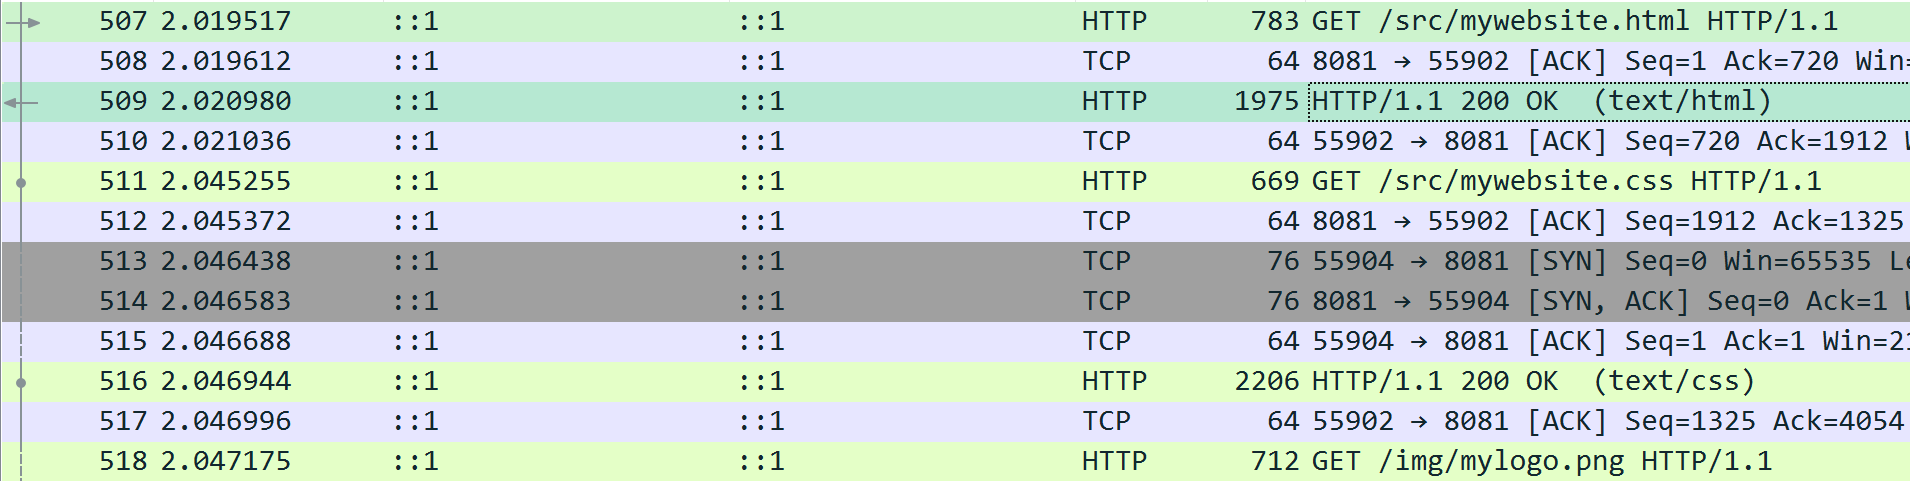
\includegraphics[width=0.8\textwidth]{img/后续请求.png}
    \caption{后续请求}
\end{figure}
在这里,可以看到浏览器又开了一个端口,三次握手建立 TCP 连接,加快请求资源的速度。点开返回的 CSS文件,可以看到响应体中的源代码:
\begin{figure}[H]
    \centering
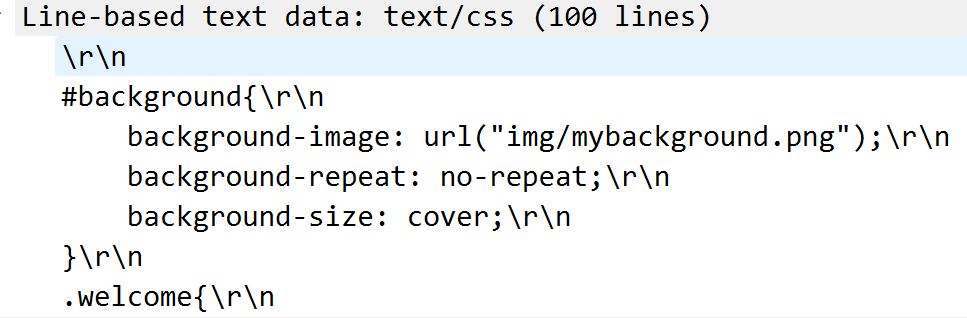
\includegraphics[width=0.6\textwidth]{img/CSS源代码.png}
    \caption{CSS源代码}
Javascipt文件类似,在此不再赘述。而对于音视频文件等非文本文件,会采用编码等技术,无法通过响应体看到有意义的信息。
\end{figure}
\begin{figure}[H]
    \centering
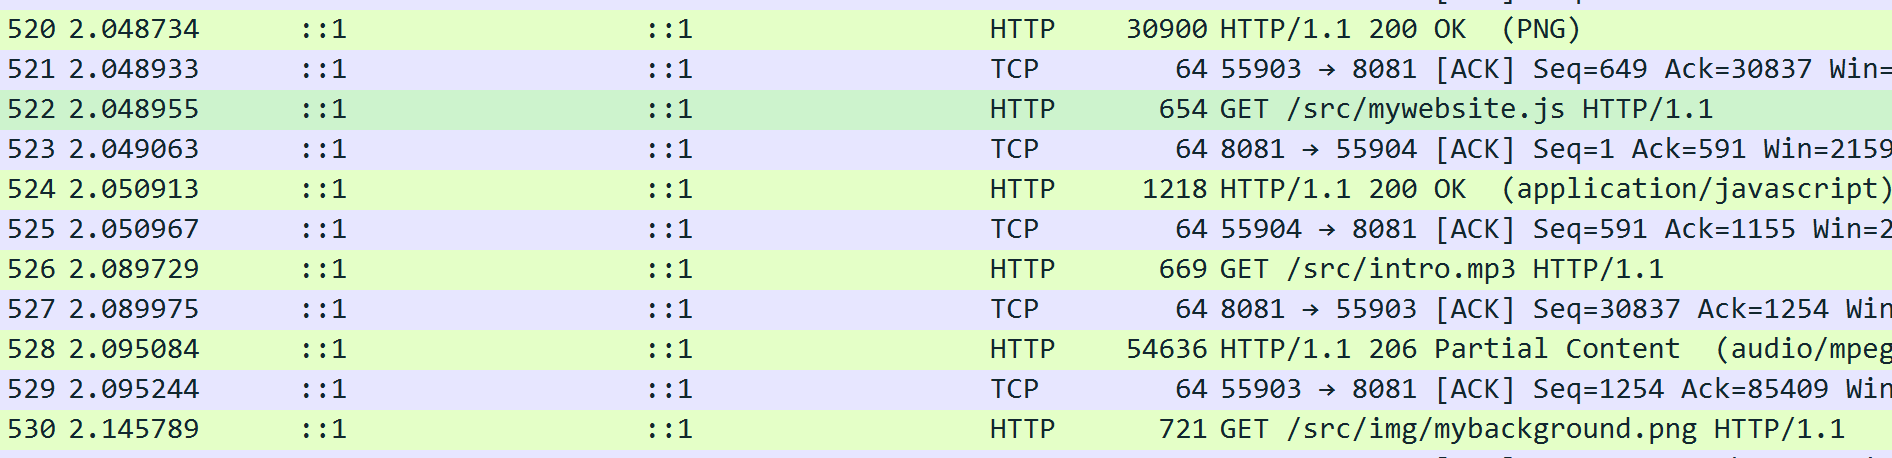
\includegraphics[width=0.8\textwidth]{img/后续请求2.png}
    \caption{后续请求2}
\end{figure}
另外发现,对于图片等比较大的文件,根据 TCP 的流量控制和拥塞控制的特点,服务端用多个TCP数据包来传输图片。
\begin{figure}[H]
    \centering
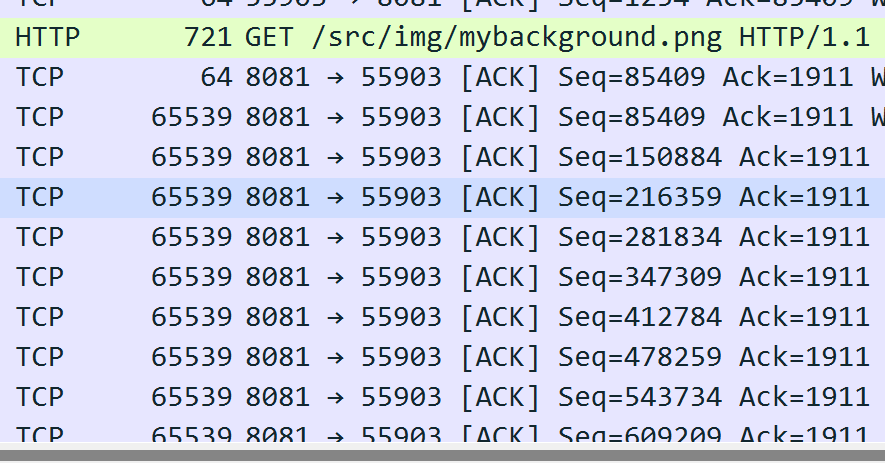
\includegraphics[width=0.6\textwidth]{img/图片传输.png}
    \caption{图片传输}
\end{figure}
最后即是 TCP 协议的四次挥手,由于有多个端口建立了 TCP 连接,所以也都需要通过四次挥手关闭连接。
\begin{figure}[H]
    \centering
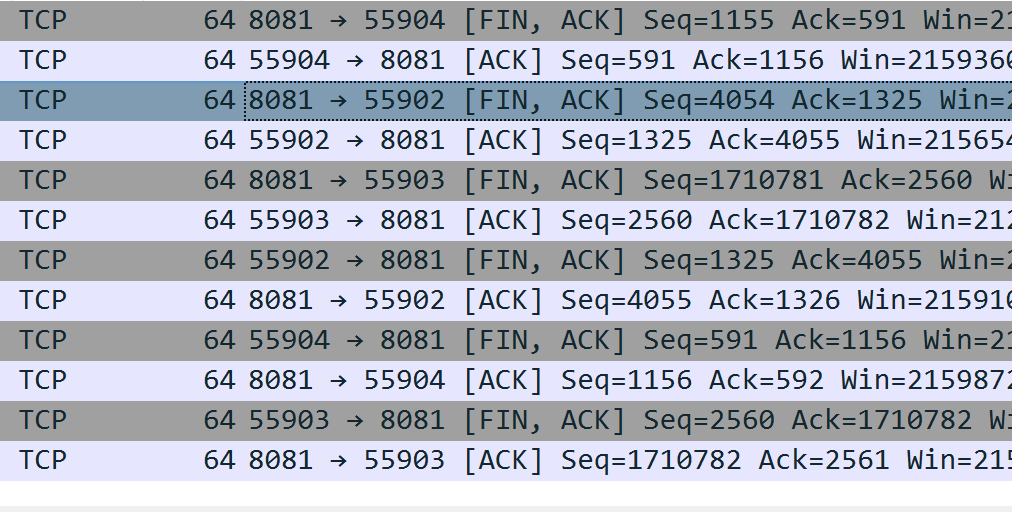
\includegraphics[width=0.6\textwidth]{img/四次挥手.png}
    \caption{四次挥手}
\end{figure}
还是以端口号55902为例来分析,但跟实验原理不同的是,是服务端首先发送 [FIN,ACK] 报文来请求关闭连接,此时 Seq=4054,而端口55902回复给服务端一个 [ACK] 报文,ACK为4055,同时设置 Seq=1325 发回给服务端;之后客户端再发送一个 [FIN,ACK] 的报文,此时 Seq=1325,ACK=4055,最后服务端发回 [ACK] 报文,Seq=4055,ACK=1326,上述的流程符合实验原理中所叙述的流程,通过四次挥手,两端成功关闭连接。至此抓包结束。

\vspace{1cm}
\section{思考与总结}
通过本次实验,我学会了使用 Apache 在本地主机上搭建Web服务器,学会了使用 HTML、CSS和 JavaScript来编写网页程序,还学会了使用 WireShark 来抓包捕获数据包,分析网络通信的过程,对 HTTP 协议和 TCP 协议的理解更加深入、更加透彻。

\end{document}
